\section{Optimization methodology}
Given an objective function $f: \mathcal{X} \rightarrow \mathbb{R}$, where the domain
$\mathcal{X}$ could be a subset of $\mathbb{R}^n$,
optimization is a methodology which seeks to find an optimal point, $x^*$, and value
$f^* = f(x)$, given as
\begin{align}\label{OPT}
    x^* \in \argmin_{x \in \mathcal{X}} f(x) \hspace{1cm} f^* = \min_{x \in \mathcal{X}} f(x) = f(x^*).
\end{align}
Note that the above formulation is a minimization problem, which is equivalent to a
maximization problem maximizing $-f(\cdot)$. Throughout this thesis, we choose to only work
with a minimization problem. 
Solving this problem (close to) exact is often intractable except for rare cases e.g. if $f$ is 
convex and analytically directly solvable or the domain of $f$ is very limited. The following example
with linear least squares is an example of such a problem. 

\begin{testexample}[Direct solution method]
    The unconstrained linear least squares, $$\min_{x\in \mathbb{R}^n} f(x) := ||Ax-b||_2^2$$
    where $A \in \mathbb{R}^{m\times n}$ and $b \in \mathbb{R}^m$, is a convex problem,
    i.e. finding $x^*$ such that $\nabla f(x^*) = 0$ is equivalent to finding the solution
    to the problem. Assuming $A^TA$ is invertable, linear least squares can be solved
    directly by the normal equations, 
    $$\nabla f(x) = 2A^TAx + 2b^TA = 0 \hspace{0.5cm} \Leftrightarrow \hspace{0.5cm} x^* = (A^TA)^{-1} A^Tb$$
\end{testexample}

Most optimization problems are non-convex with multiple local minima. And even if the gradient is
given analytically, the solution is still found among a potentially infinitely large set of
stationary points ($\nabla f(x) = 0$) and boundary points ($x \in \partial \mathcal{X}$) - this
might be tedious or impossible. Therefore, when the problem is not directly solvable, mathematical optimization
takes an indirect approach: Design a sequence of experiments that reveal information about the
objective function. This information can hopefully lead us to the solution of \eqref{OPT}. This
general way of sequentially solving is presented in the book Bayesian Optimization by Roman Garnett
\cite{bayesoptbook} and presented here as Algorithm \ref{algOPT}. 

\begin{algorithm}
\caption{Sequencial Optimization \cite{bayesoptbook} }\label{algOPT}
\begin{algorithmic}
\State \textbf{Input:} Initial dataset $\mathcal{D}$  \Comment{can be empty}
\While{Temination is not reached}
    \State $x \gets \text{policy}(\mathcal{D})$ \Comment{select next observation location}
    \State $y \gets \text{observe}(x)$ \Comment{observe objective function at chosen location}
    \State $\mathcal{D} \gets \mathcal{D} \cup \{(x,y)\} $ \Comment{update dataset}
\EndWhile
\State $\textbf{return: } \mathcal{D}$
\end{algorithmic}
\end{algorithm}

Given data points in the \textit{optimization landscape}\footnote{"Optimization landscape" defined
as the joint set of points in the domain and the objective function evaluated in the points, i.e.
$\{(x,f(x))\in \mathcal{X} \times \mathbb{R}| x \in \mathcal{X}\}$} a policy selects a location $x
\in \mathcal{X}$ where we make our next observation. Policies can be deterministic or probabilistic,
e.g. grid search and random search are policies. The next observation provides us a $y$
value, which combined with $x$ is included in the available data $\mathcal{D}$. Finally, a stopping
criterion decides whether to repeat or terminate the procedure. We will now present how different examples of
well-known optimization rutines fits into Algorithm \eqref{algOPT}.


\begin{testexample}[Grid search]
    In grid search values along each dimention in $\mathcal{X}$ is seleced and combined with each
    other, which thereby defines a parrellel grid in the optimization domain $\mathcal{X}$. All
    grid points are ordered and systematically selected. In the context of algorhtim \ref{algOPT} we define
    the grid search policy as 
    $$\text{policy}_{GS}(\mathcal{D}) = x_{|\mathcal{D}|+1}$$
    assuming $x_1,x_2, \dots, x_{m} \in \mathcal{X}$ are the ordered grid points and the size of the obtained 
    data is $|\mathcal{D}|$. Termination will happen when $|\mathcal{D}| = m$.
\end{testexample}
\begin{testexample}[Random search]
    In random search a point is randomly drawn from uniform distribution supported over the domain
    space $\mathcal{X}$, 
    $$\text{policy}_{RS}(\mathcal{D}) = x, \hspace{0.5cm} x \sim Unif(\mathcal{X})$$
\end{testexample}
\begin{testexample}[Gradient descent]
    Gradient descent (GD) is the most simple gradient-based optimization approach. The gradient of a
    continuous function points in the most ascending direction from the location where it is
    evaluated. GD uses the opposite gradient
    direction, i.e. the most descending direction, weighted with a stepsize $\eta$ to iteratively minimize the objective
    function. This yields the policy:
    $$\text{policy}_{GD}(\mathcal{D}) = x_n - \eta \nabla f(x_n)$$
    where we, for a brief moment, in Algorithm \eqref{algOPT} modify $y$ to be a vector since the observation 
    is given as:
    $$\text{observe}_{GD}(x) = [f(x), \nabla f(x)]$$
\end{testexample}

\subsection{When to use sample-efficient optimization}
Note that grid search, random search, and gradient descent are policies that entirely ignore the
available data. Ignoring potentially valuable information is a shame if the objective function is
expensive to evaluate. And indeed, improvements of the gradient descent algorithm, such as momentum
and quasi-newton methods, indirectly remember and exploit obtained data, $\mathcal{D}$. They are
examples of so-called \textit{sample-efficient} solvers since they need fewer $y$-samples to
minimize $f(\cdot)$. Choosing a more sample-efficient solver costs extra
time/energy to store and exploit the collected information for every iteration. In the end, solving
the optimization problem can be divided into the following components, 

\begin{itemize}[noitemsep]
    \item $N_{\text{iter}}$: number of iterations to reach an acceptable solution. This number depends on the
    solver. If $N_{\text{iter}}$ is relatively small, the solver is called sample-efficient. 
    \item $C_{\text{policy}}$: The solvers cost per iteration, i.e. what is the cost of calculating
    $\text{policy}(\mathcal{D})$, where cost is typically in terms of time and power usage. 
    \item $C_{\text{observe}}$: Cost per evaluation of the objective function, i.e. the cost of $\text{observe(x)}$,
    which can be in terms of money, human resources, simulations etc.
\end{itemize}
Assuming same cost pr iterations and for all evaluations, the total optimization cost, $C_{\text{total}}$, is given as 
$$C_{\text{total}} = N_{\text{iter}} \cdot \left[ C_{\text{policy}} + C_{\text{observe}}\right]$$

A sample efficient solver has a large $C_{\text{policy}}$ but a small $N_{\text{iter}}$, whereas a
simple optimization scheme like random search has a very small $C_{\text{policy}}$ but a large
$N_{\text{iter}}$. Choosing the right optimization solver depends highly on $C_{\text{observe}}$.
For small $C_{\text{observe}}$ it is favorable to find a good trade-off between $N_{\text{iter}}$
and $C_{\text{policy}}$: In deep learning the solver Adam is very popular, due to its cheap
but advanced policy \cite{}. This project deals with a dominating observation cost, i.e. the cost of the policy is assumed
neglectable $C_{\text{observe}}>>C_{\text{policy}}$. So finding a cheap policy is not relevant, focus is on
the number of iterations to reach the minima $N_{\text{iter}}$. 

\begin{testexample}[Surrogate-based optimization]
    %<SVR> <Radial Basis function> <Polynomal model/respons surface>
    In surrogate-based optimization all available data is fitted by a cheap-to-evaluate
    approximation to the objective function - this approximation is called a \textit{surrogate
    model}, $f_{\text{sur}}(x)$. Examples of surrogate models could be a neural network or a random forest. The next
    point is chosen as the point where the surrogate model is minimized. 
    $$\text{policy}_{\text{sur}}(\mathcal{D}) = \min_x f_{\text{sur}}(x)$$
    where $f_{\text{sur}}(x) \approx f(x)$ for $x$ close to the data $\mathcal{D}$. And we hope the approximation
    holds for $x$ far away from the the data.
\end{testexample}

\begin{figure}[H]%
    \centering
    {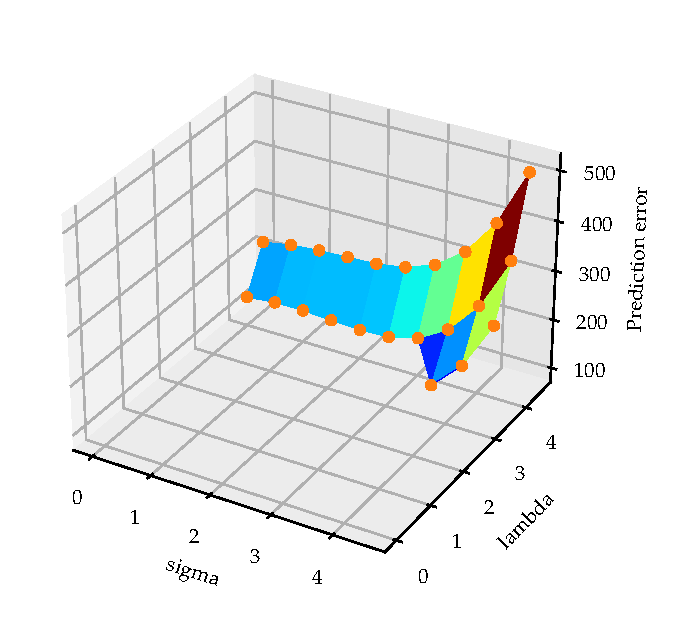
\includegraphics[width=0.46\textwidth]{Pictures/BO_vs_Grid2.eps} }%
    \qquad
   {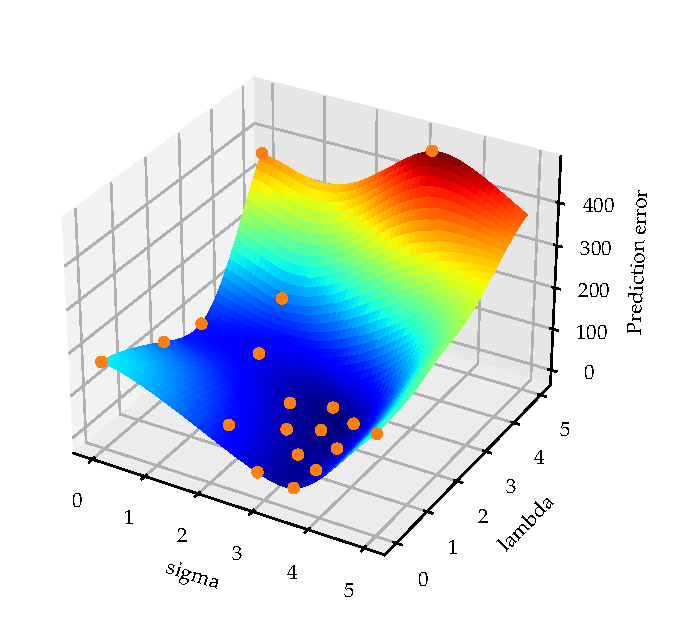
\includegraphics[width=0.46\textwidth]{Pictures/BO_vs_Grid1.eps} }%
    \caption{Example of an optimization task tuning a parameterised regression model with parameters
    $\lambda$ and $\sigma$, on a test set, i.e. minimization of prediction error. We see the first
    23 evaluations out of 100 in grid search vs 23 evaluations using a sample-efficient solver (Bayesian
    optimization). This illustrates the idea of a sample-efficient solver}%
    \label{fig:example}%
\end{figure}


\subsubsection{Noisy objective functions}
Many optimization algorithms assume \textit{exact} evaluations of the objective function. However,
this assumption is often wrong, especially for objective functions with real-life experiments,
imperfect simulations, human interaction where measurement noise is well known. A potentially noisy
objective function is the main reason why we in Algorithm \eqref{algOPT} use the terminology
$\text{observe}(x)$ and not just \textit{evaluate }$f(x)$.

The observation model is typically noisy and described as
$$y = f(x)+\epsilon$$ where $\epsilon$ is the measurement error, this is
typically assumed to be Gaussian with zero mean and a variance
$\sigma^2$ (which could depend on $x$ in a heteroskedastic setting) and implies a Gaussian observation model, 
$$p(y|f(x),\sigma^2) = \mathcal{N}(y|f(x),\sigma^2)$$ 

% (note from now on we define $\phi := f(x)$ in order to avoid confusion and a extra set of paranteses)
% $$p(y|x,\phi,\sigma) = \mathcal{N}(y;\phi,\sigma^2)$$ 

\begin{note}
    \textbf{"Sample" or "evaluate" objective function} 
    The terminology \textit{to sample} is refering to a probabilistic observation model. Formally, we
    can extend this model to deal with noiseless observations as well, simply by setting
    $\sigma = 0$ and letting the model colaps into a Direct delta distribution, $p(y|f(x)) =
    \mathcal{\delta}(y-f(x))$, i.e. all probability mass for $y$ is on the value $f(x)$ giving the
    observation sample $y = f(x)$. 
\end{note}

Bayesian optimization or probabilistic surrogate-based optimization deals with both noiseless and noisy objective functions,
as it defines a Bayesian regression model over the observations.

% \begin{figure}[h]
%     \centering
%     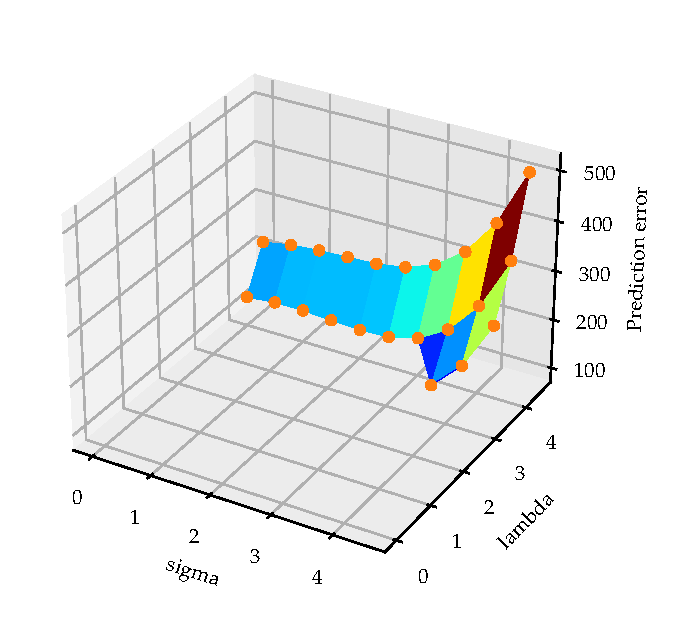
\includegraphics[width=0.9\textwidth]{Pictures/BO_vs_Grid2.eps}
%     \caption{Hyper parameter tuning of a model $M(\lambda, \sigma)$, 
%     35 evaluation in grid search vs 39 evaluations using Bayesian optimization}
%     \label{optimhist}
% \end{figure}
\begin{tcolorbox}[
    sharp corners,
    boxrule=0mm,
    enhanced,
    borderline west={4pt}{-2pt}{darkred},
    borderline north={1pt}{0pt}{darkred},
    borderline south={1pt}{0pt}{darkred},
    borderline east={1pt}{0pt}{darkred},
    %colframe=darkred!0,
    %colback=darkred!10,
    %coltitle=darkred,
    %boxsep=3pt,left=4pt,right=4pt,top=2pt,bottom=2pt
]
{ \textcolor{darkred}{\textbf{Example: Bayesian Optimization}}}\\
    Bayesian optimization is a \textit{probabilistic} surrogate-based optimization
    methodology. Here a cheap probabilistic regression model $p(y|x)$ is fitted to the
    the observations $\mathcal{D}$ and in contrast to (deterministic) surrogate-based
    optimization, it is not possible right away to find the minima in the cheap
    surrogate model; first, we need to interpret the meaning of minima in a probabilistic
    regression model. This interpretation is done through a so-called acquisition
    function (more about this later). The policy is as following,
    $$\text{policy}_{BO}(\mathcal{D}) = \max_x AQ(p(y|x,\mathcal{D}))$$

    \begin{figure}[H]
        \begin{minipage}[c]{0.67\textwidth}
          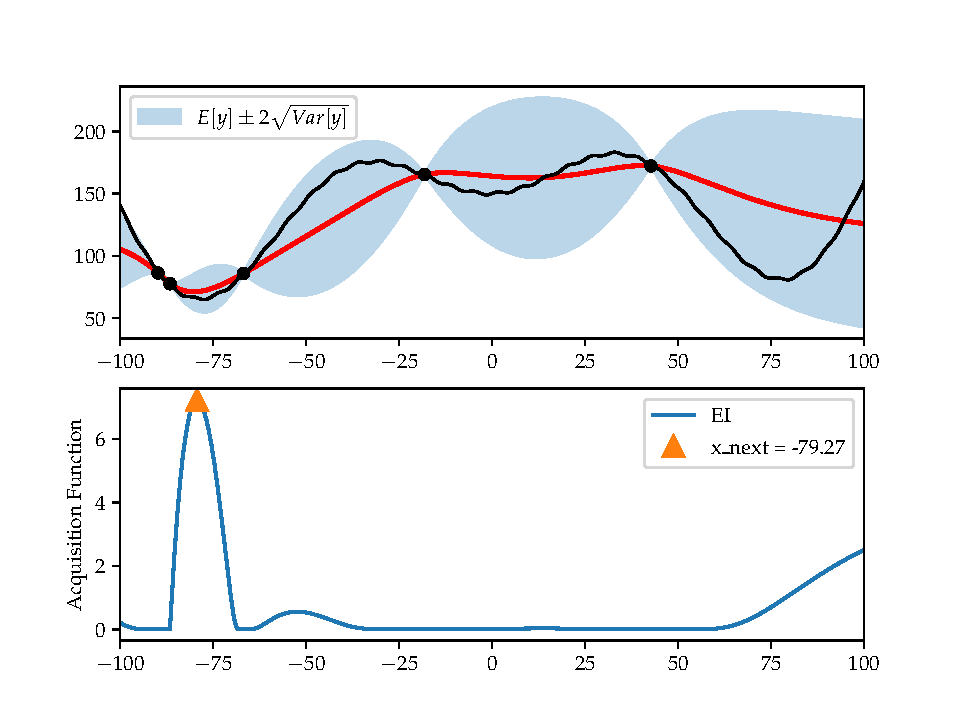
\includegraphics[width=\textwidth]{Pictures/Test1Gaussian_Process_-_sklearn000.pdf}
        \end{minipage}\hfill
        \begin{minipage}[c]{0.3\textwidth}
          \caption{Top: Bayesian regression model (Gaussian Process) is fitted to the observed data,
          which are sampled from the underlying black objective. Bottom: The expected improvement
          \textit{acquisition function} is maximied at the orange arrow, i.e. the location of the
          next sample.  $\text{policy}_{BO}(\mathcal{D}) = -79,27$} \label{fig:03-03}
        \end{minipage}
    \end{figure}
   
\end{tcolorbox}


% \begin{algorithm}[H]
%     \caption{Bayesian Optimization}
%     \begin{algorithmic}
%     \State \textbf{Input:} Initial dataset $\mathcal{D}$, Bayesian regression model.
%     \While{Temination is not reached}
%         \State Fit Bayesian regression model: $$p(y|x,\mathcal{D}) = \int p(y|x,\theta)p(\theta|\mathcal{D})d\theta$$
%         \State $x \gets \max_x AQ(p(y|x,\mathcal{D}))$\Comment{Find point with highest acquisition}
%         \State $y \gets \text{observe}(x)$ \Comment{observe objective function at chosen location}
%         \State $\mathcal{D} \gets \mathcal{D} \cup \{(x,y)\} $ \Comment{update dataset}
%     \EndWhile
%     \State $\textbf{return: } \mathcal{D}$
%     \end{algorithmic}
% \end{algorithm}


% \begin{mybox}{darkred}{A red box}
%     Test
% \end{mybox}